
Wie im vorherigen Kapitel beschrieben, existieren verschiedene Varianten, einen \gc Tausch 
durchzuführen. Für das Finden der gemeinsamen Nachbarschaft betrachten wir sieben verschiedene Methoden, 
für das Tauschen der Nachbarschaft zwei und weiterhin prüfen wir noch, ob es sinnvoll ist, 
die \red{vorsortiert} Invariante zu nutzen oder nicht, was ebenfalls zwei Möglichkeiten entspricht.
Kombiniert man all diese Möglichkeiten erhält man also insgesamt 28 verschiedene Varianten für einen \gc 
Tausch.
In diesem Kapitel diskutieren wir, welche der Varianten ausgewählt wurde.
%%%%%%%%%%%%%%%%%%%%%%%%%%%%%%%%%%%%%%%%%%%%%%%%%%%%%%%%%%%%%%%%%%%%%%%%
%%%%%% Aufbau
%%%%%%%%%%%%%%%%%%%%%%%%%%%%%%%%%%%%%%%%%%%%%%%%%%%%%%%%%%%%%%%%%%%%%%%%

\section{Versuchsaufbau}
Um die einzelnen Varianten auf Ihre Laufzeit zu testen, wurde eine Art Versuch aufgebaut.
Dazu wurden alle Methoden in \cpp programmiert. Diese wurden dann auf unterschiedlichen
Instanzen getestet und mittels Google Benchmark \cite{benchmark} wurde die Zeit gemessen, 
die für das Ausführen benötigt wurde.
\\
\\
\red{Google Benchmark ist ein \red{Framework} ...?}
\\
\\
Wie %\red{vorher (kapitel ..?)} 
beschrieben benötigen die Methoden als Eingabe keinen Graph, 
sondern lediglich zwei Vektoren, welche jeweils die Nachbarschaft zweier Knoten repräsentieren. Ohne 
Beschränkung der Allgemeinheit nennen wir den größeren (sofern einer der beiden Vektoren größer ist)
$u$ und den kleineren $v$.
Um möglichst gut zu erkennen, wie sich die verschiedenen Methoden bei unterschiedlichen
Eingaben verhalten, messen wir die Laufzeiten für eine ganze Reihe an Instanzen. 
Um ein gutes Bild zu erhalten, sollten folgende Fälle auf jeden Fall abgedeckt sein:

\begin{itemize}
	\item Beide Vektoren liegen in der gleichen Größenordnung
	
	\item Einer der Vektoren ist wesentlich größer als der andere
	
	\item Der Anteil an gemeinsamen Nachbarn ist groß
	
	\item Der Anteil an gemeinsame Nachbarn  ist klein
\end{itemize}
Um dies zu erreichen, \red{erstellen} wir mehrere Runden, in denen der Vektor $u$ von anfänglich 128
Elementen auf bis zu 4.000.000 Elementen vergrößert wird. Innerhalb jeder Runde werden mehrere Durchläufe 
durchgeführt, bei denen der Vektor $u$ eine Größe zwischen 32 Elementen und der jeweiligen Größe von $v$ hat.
Für jeden dieser Durchgänge werden die beiden Vektoren mit zufälligen, aber paarweise verschiedenen,
Werten befüllt, bis sie die entsprechende Größe haben. 
Dabei haben die Vektoren aber offensichtlich keine Elemente gemeinsam, was dazu führen würde, dass ein \gc 
Tausch nichts verändern würde. Um sicherzugehen,
dass die gemeinsamen Nachbarschaft nicht leer ist, müssen somit Elemente des einen Vektors 
in den anderen hineinkopiert werden. Damit die Größe der gemeinsamen Nachbarschaft
variiert wird, werden zuerst 10, dann 25, 50 und 75 Prozent der Elemente kopiert. 
\\
Eine einzelne Test Messung lässt sich somit durch ein Tripel \fett{(\la, \sm, \fr)} beschreiben, wobei
\fett{\la} die Größe von $u$ ist, \fett{\sm} die Größe von $v$ und \fett{\fr} der Anteil der gemeinsamen Elemente.





%%%%%%%%%%%%%%%%%%%%%%%%%%%%%%%%%%%%%%%%%%%%%%%%%%%%%%%%%%%%%%%%%%%%%%%%
%%%%%% Messung
%%%%%%%%%%%%%%%%%%%%%%%%%%%%%%%%%%%%%%%%%%%%%%%%%%%%%%%%%%%%%%%%%%%%%%%%

\section{Messung}
Auf die im vorherigen Abschnitt beschriebene Weise, werden die verschiedenen Instanzen erstellt und
mittels Google Benchmark die Zeit gemessen. Aus Zeitgründen werden jedoch nicht alle Werte 
für \la{} und \sm{} erstellt. Deshalb verdoppeln wir in jedem Schritt die Werte von \la{} und \sm{}
anstatt sie um eins zu inkrementieren. Somit wurde für insgesamt 672 Instanzen die Laufzeit der 
einzelnen Methoden gemessen. Die Dauer für alle 28 Varianten hat dabei in Summe ungefähr 19 Stunden betragen.          
\\
\red{benchmark mintime..?}
\red{Um eventuelle Messfehler zu minimieren, wird jeder Durchlauf durch Google Benchmark 5 mal wiederholt.
}
\\
Alle Messungen wurden \red{auf einem Rechner} mit \red{64GB} Arbeitsspeicher und 16 Prozessoren vom Typ Intel(R) Xeon(R) CPU E5-2630 v3 @ 2.40GHz,
welche jeweils 8 Kerne und einen Cache von 20 MB haben, ausgeführt.


%%%%%%%%%%%%%%%%%%%%%%%%%%%%%%%%%%%%%%%%%%%%%%%%%%%%%%%%%%%%%%%%%%%%%%%%
%%%%%% Auswertung
%%%%%%%%%%%%%%%%%%%%%%%%%%%%%%%%%%%%%%%%%%%%%%%%%%%%%%%%%%%%%%%%%%%%%%%%

\section{Auswertung}
\red{mit hilfe von Jupyter notebook ausgewertet... daten aus json file }

Die erhaltenen Messdaten werden schließlich mit dem \red{Tool} Jupyter Notebook ausgewertet.
\\
\\
\\
\begin{figure}[h]
\centering
	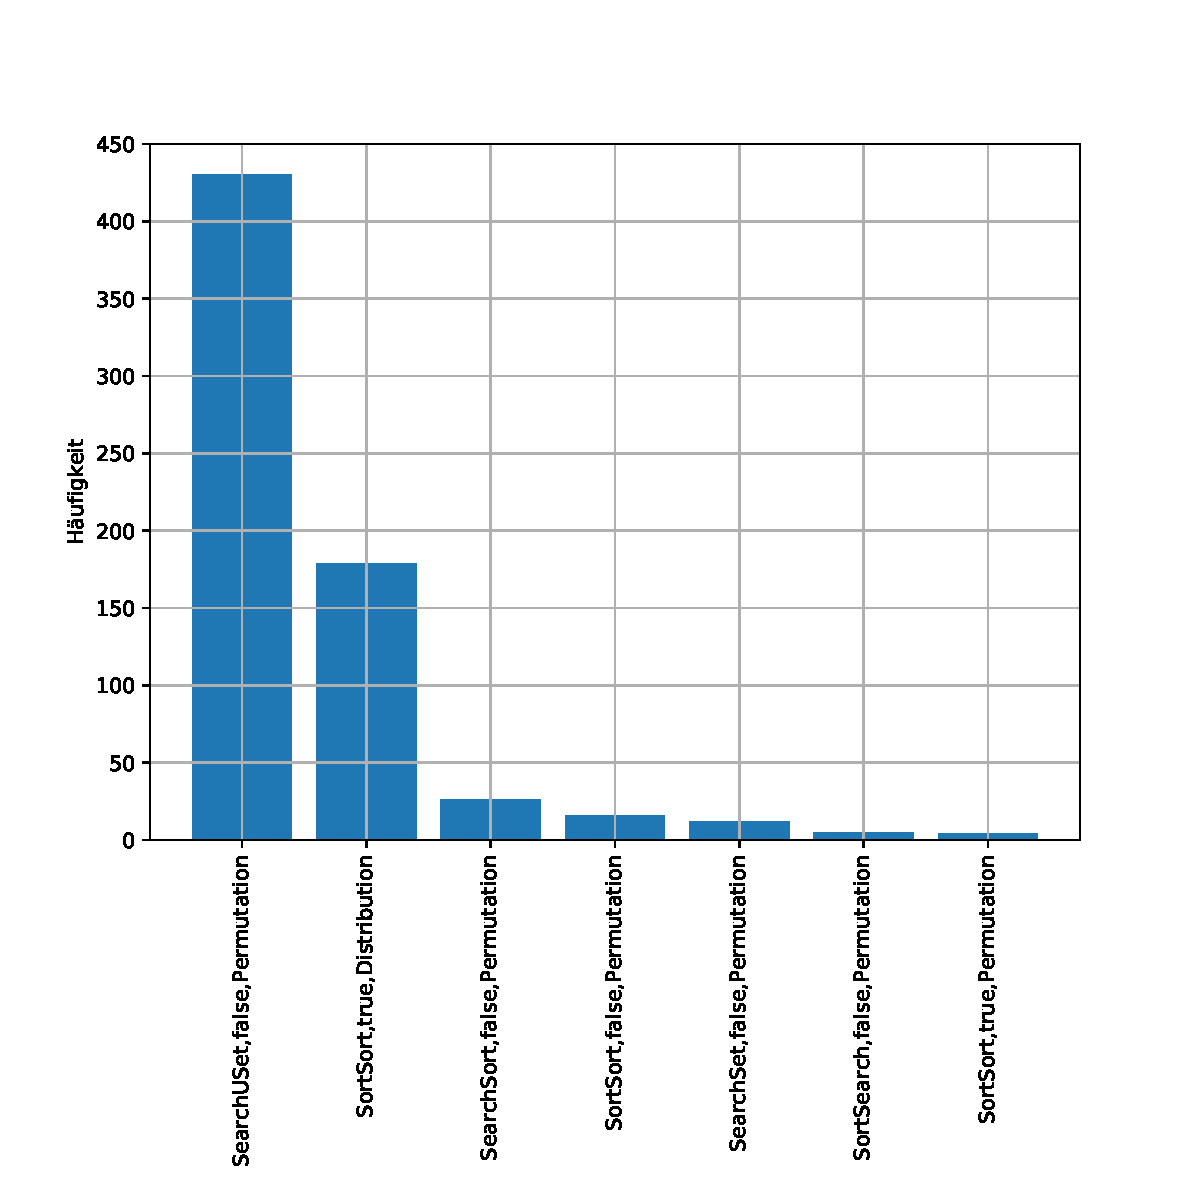
\includegraphics[width = 0.5\textwidth]{figures/counting.pdf}
	\caption{\red{Häufigkeit} \red{HIER KEIN FLOAT?}}
	\label{fig:messung_counting}
\end{figure}
Zuerst betrachten wir für jede Instanz, welche Methode am schnellsten war, also für welche die geringste
Laufzeit gemessen wurde. Interessant sind dann jeweils die Methoden, die häufig am schnellsten waren.
In Abbildung \ref{fig:messung_counting} ist dazu ein Balkendiagramm gegeben.
Dabei sieht man eindeutig, dass die Variante (\SeaUSet,\false,\perm) mit Abstand 
auf den meisten Instanzen die schnellste Laufzeit aller Methoden hat. Die
430 Instanzen, auf denen (\SeaUSet,\false,\perm) die schnellste Methode ist, entsprechen einem Anteil von rund
64\%. Mit 179 \glqq gewonnenen\grqq Instanzen folgt die Variante (\SorSor,\true,\distr), was einem Anteil von
27\% entspricht. Zusammen ist somit in etwa 91\% aller getesteter Instanzen eine dieser beiden Methoden
die schnellste gewesen. Daher liegt der Schluss nahe, sich beim Suchen der \glqq besten\grqq{} Variante,
auf diese beiden Methoden zu beschränken. Um nicht fälschlicherweise \glqq gute\grqq{} Methoden auszuschließen
betrachten wir einen weiteren Plot in Abbildung \ref{fig:messung_slowdown}. 
\begin{figure}[h]
\centering
	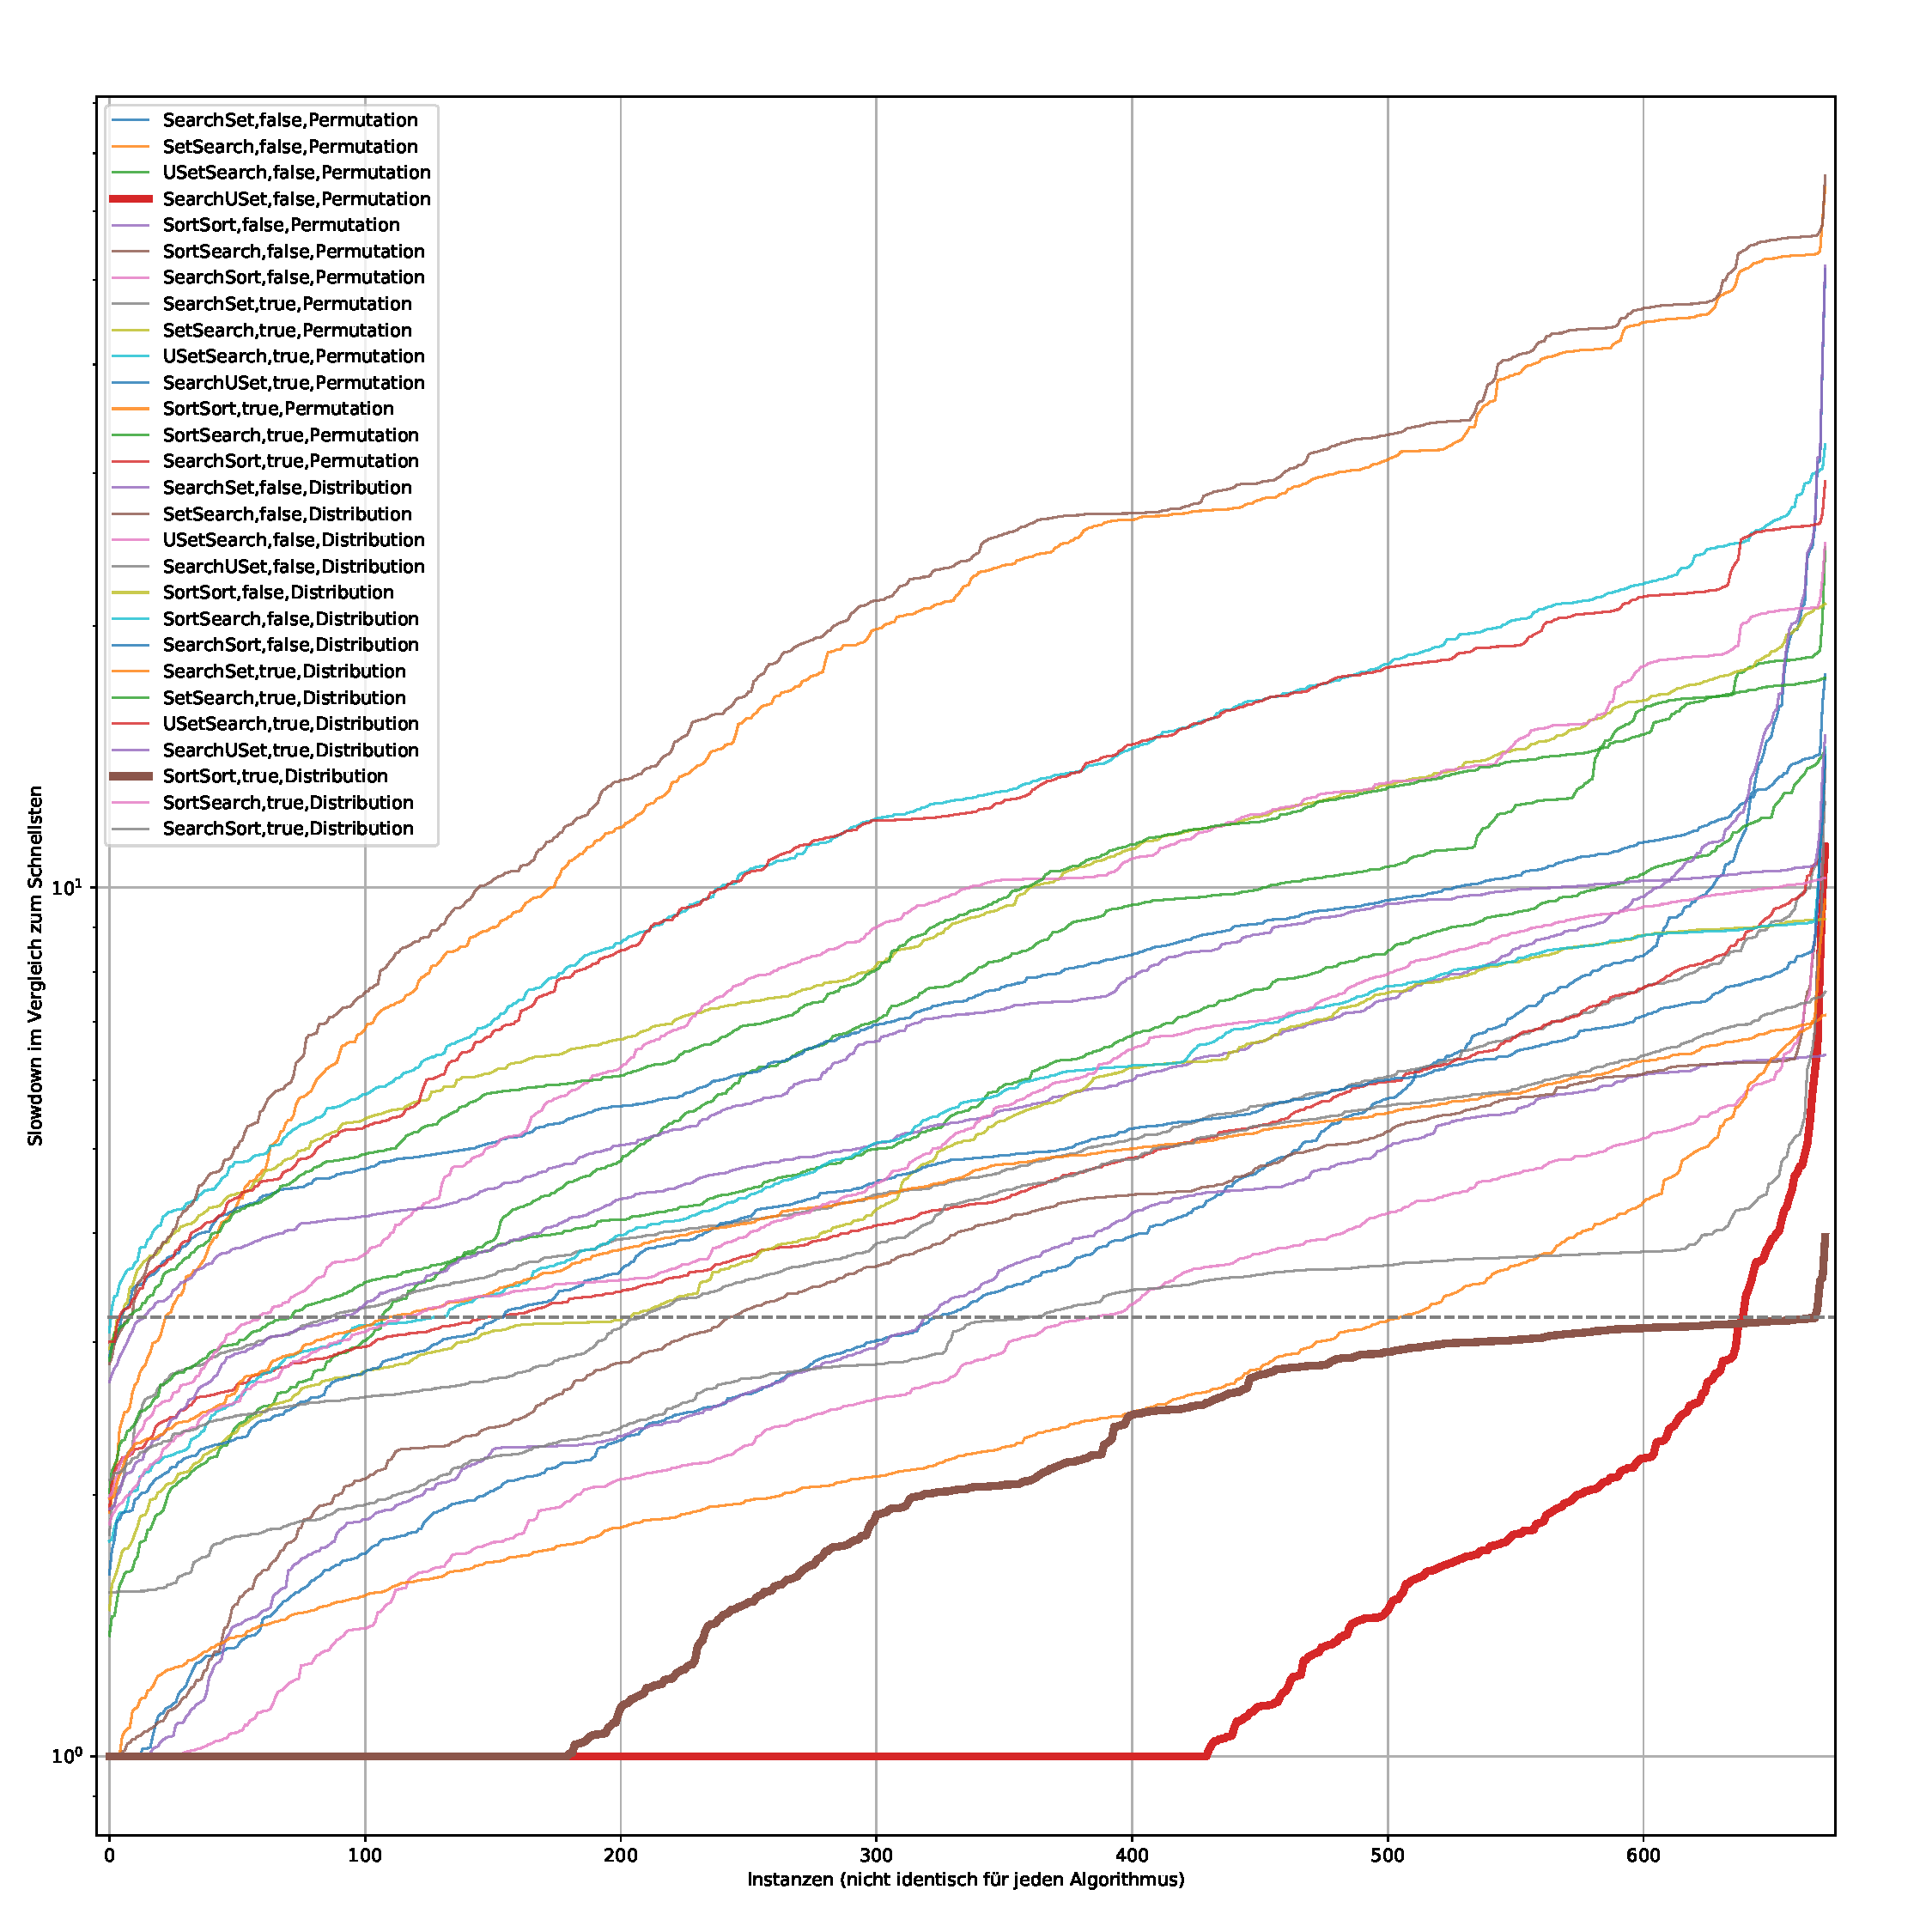
\includegraphics[width = 0.8\textwidth]{figures/slowdown.pdf}
	\caption{\red{Slowdown}}
	\label{fig:messung_slowdown}
\end{figure}
Um diesen Plot zu erstellen wurde jede Variante einzeln betrachtet.
Dann wird für jede Instanz bestimmt, welche Variante die kürzeste Laufzeit hat und der Quotient
aus dieser Laufzeit und der Laufzeit der betrachteten Variante berechnet. Dieses Verhältnis wird als \red{Slowdown}
bezeichnet und gibt an, um welchen Faktor die Variante langsamer als die schnellste ist. Die Slowdowns
zu jeder Instanz werden schließlich aufsteigend sortiert und als \red{Kurve} in den Plot eingefügt.



\red{Durch das sortieren geht die ordnung verloren}



Dieser Plot legt ebenfalls nahe, sich auf die beiden Varianten (\SeaUSet, \false, \perm) und 
(\SorSor, \true, \distr) zu konzentrieren, da die beiden Kurven am wenigsten stark \red{wachsen} und damit 
die Slowdowns vergleichsweise klein sind. Jedoch lässt sich auch hier nicht bestimmen, welche der beiden
Varianten die bessere ist. Ein Vorteil von (\SeaUSet, \false, \perm) ist, 
dass die Methode auf den meisten Instanzen einen Slowdown
von eins hat -- was wir ja auch schon in Abbildung \ref{fig:messung_counting} gesehen haben --
und damit langsamer anwächst. Ein Nachteil liegt aber darin, dass der Slowdown für manche Instanzen
eine Größe von bis zu 10.0 erreicht, während der Slowdown von  (\SorSor, \true, \distr) durch den maximalen
Wert von 3.5 beschränkt ist (in Abbildung \ref{fig:messung_slowdown} als gestrichelte Linie eingezeichnet).
\\
Dieser Nachteil spiegelt sich ebenfalls in Abbildung \ref{fig:messung_mean} wieder. In diesem Plot
wurden über alle Instanzen für jede Variante jeweils die mittlere Laufzeit bestimmt. Obwohl
es nicht in den meisten Fällen die schnellste Variante ist, hat (\SorSor, \true, \distr) die 
kleinste mittlere Laufzeit mit rund 0.0387 Sekunden. Auf Platz zwei folgt
(\SeaUSet, \false, \perm) mit etwa 0.0640 Sekunden, was schon einer Abweichung von ungefähr 60\% entspricht.
Auch in diesem Plot sieht man deutlich, dass es sich nicht lohnt noch weiter Varianten zu betrachten. Zwar hat 
auch (\SorSor, \true, \perm) eine mittlere Laufzeit, die annähernd so groß ist wie (\SeaUSet, \false, \perm),{}
die aber \red{nicht an die schnellste herankommt}. Alle anderen Varianten haben eine deutlich größere mittlere
Laufzeit.
\begin{figure}[h]
\centering
	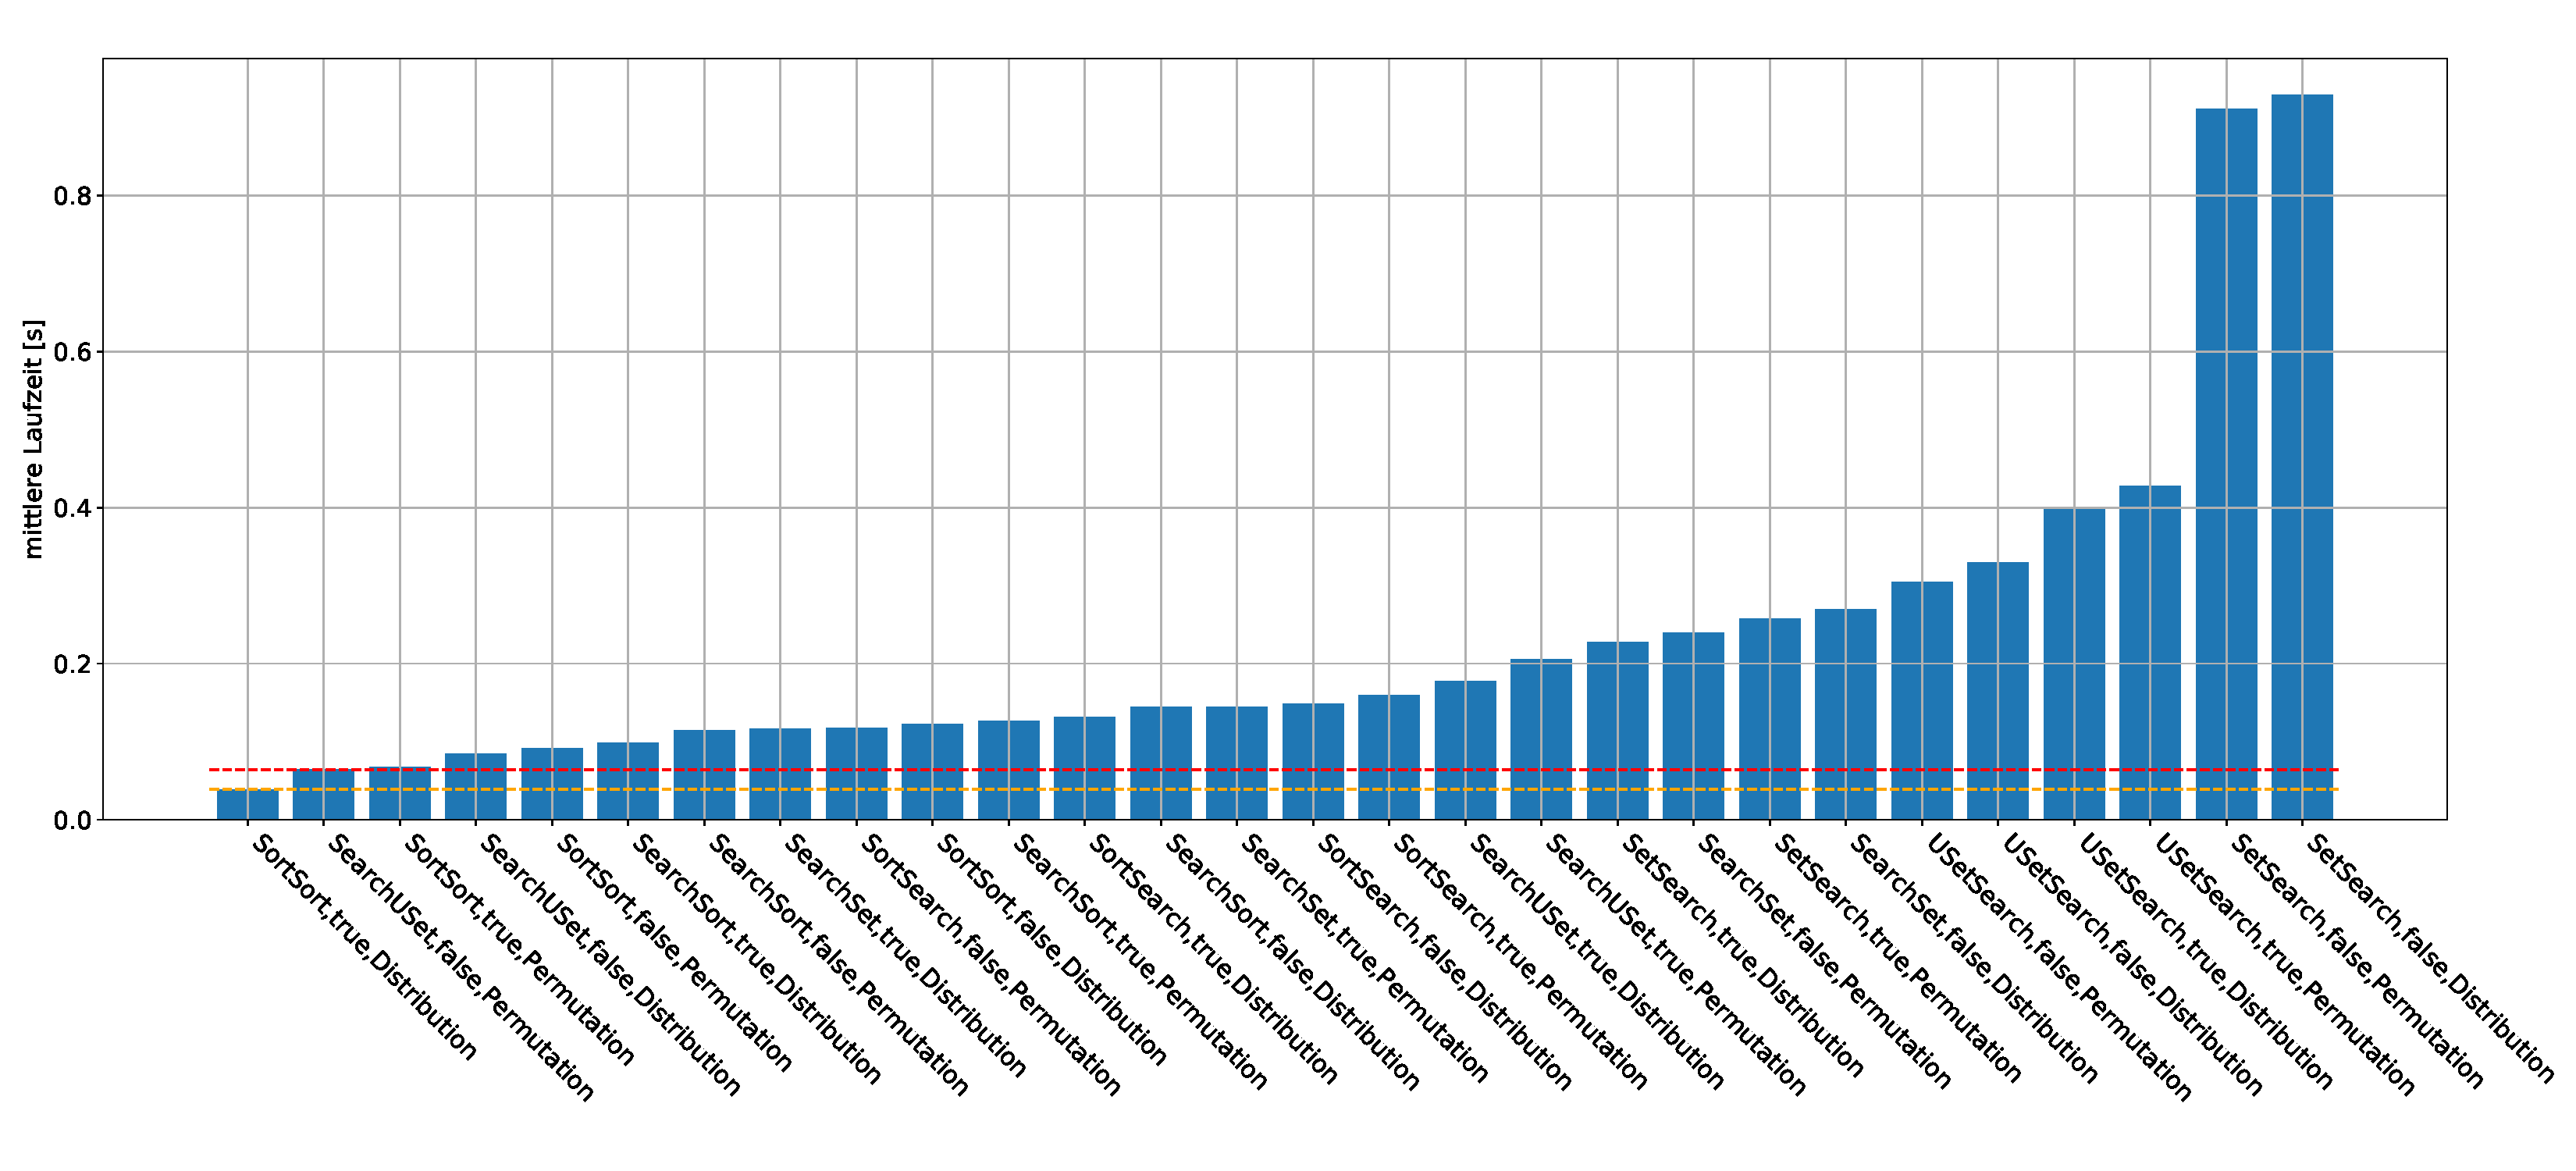
\includegraphics[width = \textwidth]{figures/mean.pdf}
	\caption{Mittlere Laufzeiten der Varianten über allen Instanzen}
	\label{fig:messung_mean}
\end{figure}
Abschließend betrachten wir noch die zwei ausgewählten Varianten im direkten Vergleich. Dazu wurden
in Abbildung \ref{fig:messung_small} auf der horizontalen Achse die getesteten Instanzen aufgetragen
und dazu die jeweiligen Laufzeiten von (\SorSor, \true, \distr) und (\SeaUSet, \false, \perm) als Kreuze
eingezeichnet. Die Instanzen sind nach aufsteigenden Werten für \sm{} sortiert. Aus Gründen der Übersichtlichkeit
wird bei  der Beschriftung der Instanzen der Teil \fr weggelassen, die Instanzen werden 
nur mit \la, \sm{} bezeichnet. Weiterhin wurden der
Übersichtlichkeit wegen die Instanzen aus dem Bereich $32 < \text{\sm}  <32768$ ausgelassen, da sie das gleiche
Bild wie die üblichen Instanzen zeigen.
Man sieht dabei, dass sich die Laufzeiten in den meisten Instanzen nicht so stark unterscheiden.
Dies sind vor allem die Instanzen, bei denen der Unterschied zwischen \la{} und \sm{} nicht so groß ist.
In den Instanzen, in denen sich die Werte für \sm{} und \la{} stark unterscheiden, ist jedoch ein 
deutlicher Vorteil von (\SorSor, \true, \distr) zu erkennen. Auch bei den \glqq großen\grqq{} Instanzen
mit Werten von $\text{\sm{}}> 500.000$ hat diese Variante einen deutlichen Laufzeitvorteil.
Auf der Instanz (4.194.304, 4.194.304, 75) beispielsweise hat (\SeaUSet, \false, \perm) eine Laufzeit
von circa 1.628 Sekunden, während (\SorSor, \true, \distr) nur etwa 0.146 Sekunden benötigt. Der Slowdown
beträgt für diese Instanz also in etwa 11. 
\begin{figure}[h]
\centering
	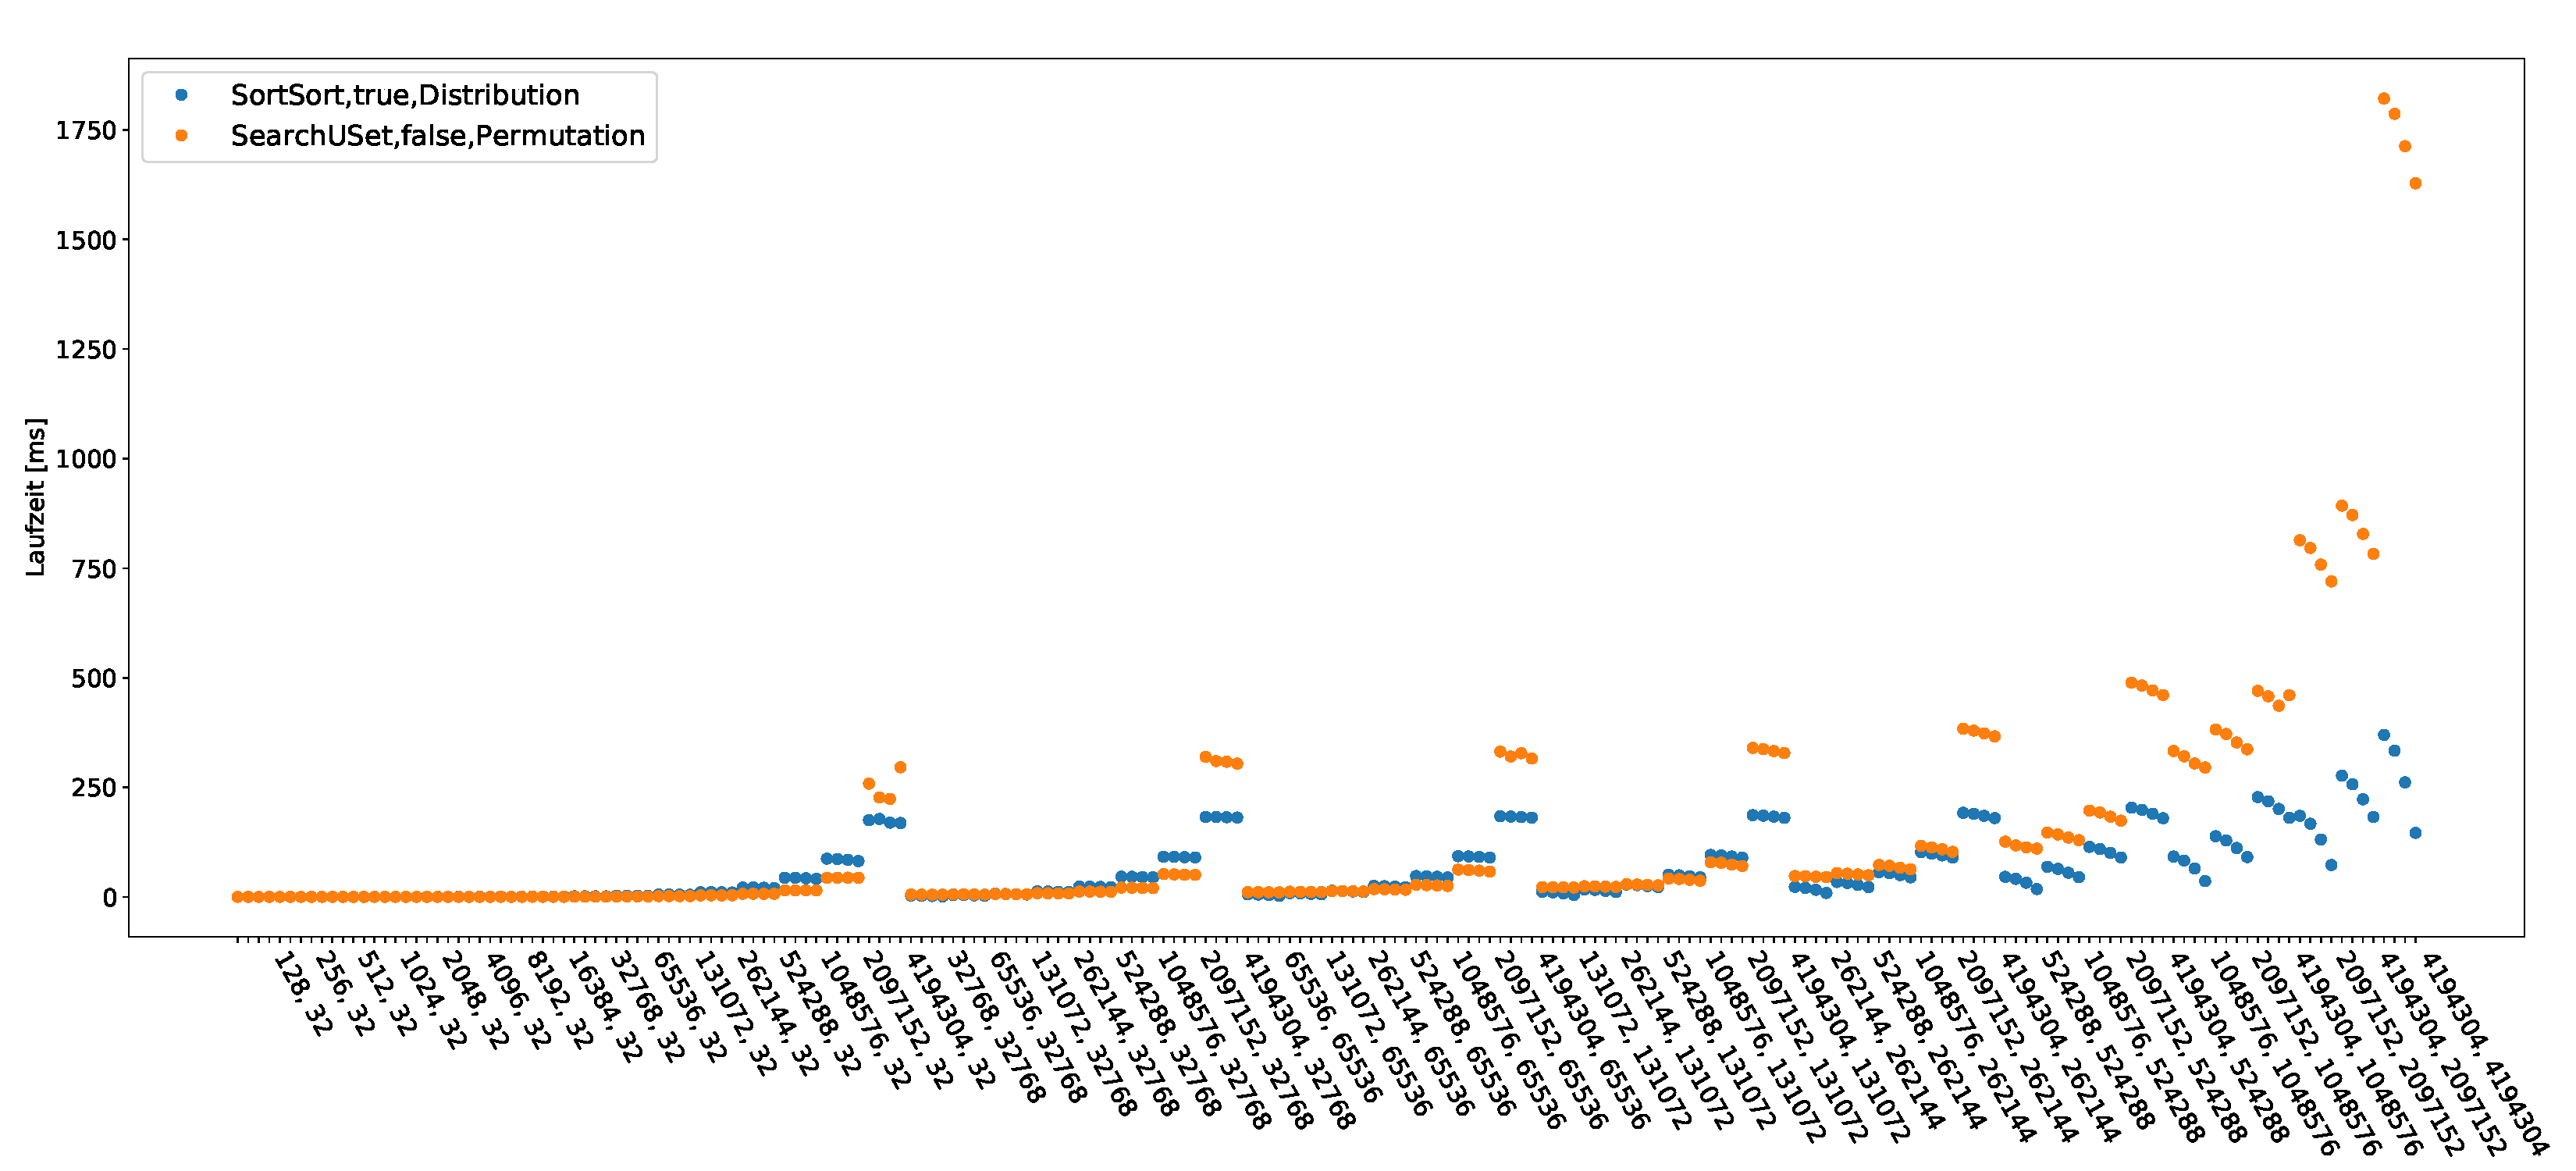
\includegraphics[width = \textwidth]{figures/small_aufsteigend.pdf}
	\caption{\red{kleines aufsteigend}}
	\label{fig:messung_small}
\end{figure}


%%%%%%%%%%%%%%%%%%%%%%%%%%%%%%%%%%%%%%%%%%%%%%%%%%%%%%%%%%%%%%%%%%%%%%%%
%%%%%% Fazit
%%%%%%%%%%%%%%%%%%%%%%%%%%%%%%%%%%%%%%%%%%%%%%%%%%%%%%%%%%%%%%%%%%%%%%%%

\section{\red{Fazit}}
Abschließend muss an Hand der Messdaten entschieden werden, welche Variante zum Einsatz für
einen \ct am Besten geeignet ist.
Zusammenfassend haben wir im vorherigen Abschnitt festgestellt, 
dass nur die Varianten (\SorSor, \true, \distr) und (\SeaUSet, \false, \perm) zur Auswahl stehen.
Während die eine Variante am häufigsten die geringste Laufzeit hat, liegt die andere 
bei der durchschnittlichen Laufzeit weiter vorne. Dies liegt vor allem daran, dass sich 
die Laufzeiten bei den Instanzen auf denen (\SeaUSet, \false, \perm) \glqq gewinnt\grqq{} kaum unterscheiden.
Unter den anderen Instanzen gibt es jedoch welche, bei denen (\SorSor, \true, \distr) bis auf einen
Faktor von circa 11 schneller ist.
\\
Um ein bestmögliches Laufzeitverhalten für einen \ct zu erreichen, könnte man auf die Idee kommen, 
beide Varianten zusammen zu nutzen. Man könnte sich eine \red{Heuristik} überlegen, die jeweils angibt, 
auf welcher Instanz man welche Variante verwenden sollte. Somit würde bei jedem \ct abhängig von 
der Eingabe, also den Nachbarschaften, entschieden werden, welche der beiden Instanzen man benutzt. 
Das Problem dabei liegt jedoch darin, dass bei diesen Varianten einmal die Vorsortiert-Invariante
genutzt wird und einmal nicht. Dies ist natürlich nicht beides gemeinsam möglich. Entweder man hält die
Nachbarschaften immer sortiert, oder eben nicht. Man muss sich also für eine Möglichkeit der
Invariante entscheiden. Dadurch ändert sich dann aber zwangsläufig  eine der beiden Varianten. 
Entscheidet man sich, die Nachbarschaften sortiert zu halten, würde (\SeaUSet, \false, \perm) zu (\SeaUSet, \true, \perm){}
werden, andernfalls würde sich (\SorSor, \true, \distr) zu (\SorSor, \false, \distr) verändern.
Diese beiden \glqq veränderten \grqq{} Varianten haben aber jeweils deutlich schlechtere Laufzeiten
als die ursprünglichen.
\\
Es ist also nicht sinnvoll möglich, die beiden Varianten miteinander zu kombinieren. Wir müssen uns
also auf eine Variante festlegen. Dies ist die Variante (\SorSor, \true, \distr), da sie im Vergleich zur
Alternative -- wie schon beschrieben --
in kaum einer Instanz eine wesentlich schlechtere Laufzeit hatte, jedoch auf manchen Instanzen wesentlich
bessere Laufzeiten. Außerdem ist es die Variante mit der geringsten mittleren Laufzeit. 
Ein Vorteil dieser Variante neben der Laufzeit liegt noch in der Einfachheit. So werden
lediglich die beiden Arrays sortiert und linear durchlaufen. Es muss keine weitere Datenstruktur
erstellt werden -- wie bei der anderen Variante das \texttt{unordered\_set} -- und damit wird
auch kein zusätzlicher Speicherplatz verbraucht.

